\section{Implementation}

\subsection{Choosing a Renderer}

As discussed, to render a GPIS using light transport you need to sample ray intersections from a conditioned Gaussian process and return surface interactions like a regular light transport algorithm.

A ground-up implementation could be realized from scratch using CUDA or OpenGL compute shaders. This would involve defining scene traversal, ray intersection routines, multiple importance sampling, surface interactions, and other components, as well as scene parsing and uploading to GPU memory from the CPU. This approach would provide complete control over the renderer but also requires implementing substantial ray tracing boilerplate unrelated to GPIS.

Alternatively, we could create a custom node for a state-of-the-art renderer like Blender Cycles \cite{Blender} or Autodesk Arnold. \cite{Arnold} Both renderers use Monte Carlo path tracing for volumetric media and mesh-based assets, and they allow the creation of plugins or ``nodes'' to define custom behavior. Unfortunately, they do not provide sufficient flexibility to define custom ray intersection behavior from sampling a Gaussian process, which is essential for GPIS integration.

A third option is using research-focused renderers. Tungsten \cite{Tungsten} is the renderer used by \textcite{seyb24from,xu25practical}. It was developed by \textcite{Tungsten}, and the GPIS implementation is available on github. Although publicly available, it is not designed for public use and lacks documentation. The released version does not support loading hair files and conditioning Gaussian processes from the retrieved splines. Adding this functionality would be an interesting extension but would require reverse-engineering Bitterli's code.

Mitsuba3 \cite{Mitsuba3} is a popular option for research-based rendering. It is a retargetable renderer developed by \textcite{Mitsuba3} at EPFL. It exposes a Python API for defining custom plugins such as custom integrators or custom BSDFs. While it does not allow defining custom ray intersection routines through the Python API, this is possible by implementing a custom shape through the C++17 codebase.

Mitsuba3, being a research-oriented open-source project, makes it an good choice. Compared to the from-scratch approach, it saves time on implementing ray tracing routines. It is actively maintained and documented, unlike Tungsten, and it provides significant flexibility while supporting retargetable execution, unlike Cycles and Arnold.

\subsection{Mitsuba 3}
From the GitHub page:
\begin{quote}
Mitsuba 3 is a research-oriented rendering system for forward and inverse light transport simulation developed at EPFL in Switzerland. It consists of a core library and a set of plugins that implement functionality ranging from materials and light sources to complete rendering algorithms. Mitsuba 3 is retargetable: this means that the underlying implementations and data structures can transform to accomplish various different tasks. \cite{Mitsuba3}
\end{quote}

\subsubsection{The API}
The following is taken from the official documentation for Mitsuba 3 \cite{Mitsuba3}.

\paragraph{Plugins}
The path tracing architecture of Mitsuba is separated into components called plugins. They represent the systems needed for rendering. I will present the relevant ones for implementing a GPIS-based shape.

\paragraph{Integrator}
Integrators are responsible for defining how to solve the light transport equation. They handle scene traversal and determine the rendering strategy. Most integrators define a depth parameter that controls how many bounces the ray will perform before returning a sample. The path tracer integrator is an existing plugin and serves as a good default. It handles much of the heavy lifting of the rendering equation and implements useful optimizations such as multiple importance sampling.

\paragraph{Shapes}
Shapes define surfaces that mark the intersection between different types of materials, such as the transition between air and a solid surface. They can also define intersections with volumes like smoke. All shapes must define a bounding box, which is used by the integrator for scene traversal.

Existing shape plugins in Mitsuba include basic primitives like cubes, spheres, planes, and disks, as well as mesh-based shapes that load vertices from Wavefront (.obj) and PLY formats.

This project will require the creation of a custom shape called \texttt{gpis\_shape} that can load vertices and condition a Gaussian process. The Shape API is responsible for implementing the ray intersection routine called by the integrator. This routine returns a surface interaction object that defines how light interacted with the shape once the bounding box is crossed. 

\paragraph{BSDF}
Bidirectional Scattering Distribution Functions (BSDFs) are surface scattering models that represent how light bounces off a specific surface. The implementation of a custom BSDF should not be needed, as the scattering from the GPIS should behave exactly like a mesh-based counterpart. Therefore, the \texttt{gpis\_shape} implementation should be compatible with any BSDF. An existing hair BSDF exists that will be used, which implements the \textcite{chiang2016} model.

\paragraph{Sampler}
Samplers generate the random numbers used in Monte Carlo integration for rendering. They control the quality and distribution of samples taken during the rendering process.


\subsection{Proof of Concept}
I implemented a proof of concept by adding a \texttt{gpis\_sphere} shape plugin to the Mitsuba 3 renderer. The custom shape conditions a Gaussian process using 201 observation points: 100 surface points, 100 exterior points, and one interior point. The renderer represents the intersection with the mean of the conditioned Gaussian process. The sphere is placed in a traditional Cornell Box scene through Mitsuba's XML scene description, with walls using the existing rectangle shape and lighting provided by an area light emitter plugin.

\begin{figure}[htbp]
    \centering
    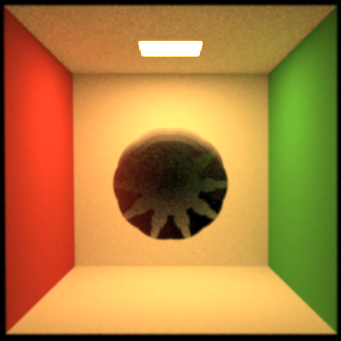
\includegraphics[width=0.7\textwidth]{img/gpis_render.png}
    \caption{Cornell Box scene with GPIS sphere rendered at 256x256 resolution using 128 samples per pixel. Render time: 30 minutes.}
    \label{fig:gpis_sphere}
\end{figure}

\subsection{Development Challenges}

\subsubsection{Build Environment Configuration}
Implementing the proof of concept presented several technical challenges. Initially, compiling Mitsuba 3 on my machine required careful environment configuration with precise version matching of dependencies. Rather than working directly on a fork of Mitsuba, I configured the system to link Mitsuba 3 as an external library to my plugin, which required understanding the Mitsuba 3 CMake compilation pipeline.

\subsubsection{Gaussian Process Library Development}
Writing the Gaussian Process helper library required multiple iterations. I first attempted to use the existing \texttt{libgp} library, but its interface did not expose the necessary functionality for sampling the Gaussian process. Next, I tried implementing a custom Gaussian library using Eigen3, but type conflicts arose with DrJit types.

DrJit is the just-in-time compiler used by Mitsuba 3, developed by the EPFL team. DrJit enables compilation to CUDA, LLVM, or scalar backends from unified source code, providing seamless parallelization optimization and automatic differentiation. However, treating the intersection routine as SIMD created conflicts with standard C++ and Eigen3 types. The solution was to implement the Gaussian process class entirely using DrJit syntax to ensure compatibility with the Mitsuba shape class interface.

Currently, \texttt{gaussian\_process.h} is a simple Gaussian process helper that enables conditioning a model from surface, exterior, and interior observations using an RBF kernel. For this proof of concept, I have not yet implemented correlated sampling from the conditioned process. Instead, the intersection routine uses a simple ray marching algorithm that searches for intersections with the mean of the process.

\subsection{Results and Analysis}

Figure~\ref{fig:gpis_sphere} shows a Cornell Box with a GPIS sphere at the center. The sphere exhibits several notable characteristics. First, the surface is not perfectly smooth and shows bumps at the conditioned points, which is expected given the sparse conditioning of only 100 surface points and the RBF kernel interpolation between them.

The lighting behavior demonstrates correct integration with Mitsuba 3's BSDF system: strong light reflection appears at the top of the sphere, while the sides reflect the wall colors. This confirms that the implementation is compatible with existing Mitsuba 3 BSDFs.

An approximation in the current implementation is the use of regular sphere normals instead of the gradient method, meaning the normals are not consistent with the actual surface orientation. I believe this inconsistency causes the black triangular artifacts at the bottom of the sphere.

The sphere also exhibits a visibly transparent appearance at the top, which is a desirable consequence of the GPIS stochastic approach. This gives confidence that this implementation can represent both hard mesh surfaces and participating media along the same continuum.

\subsection{Next Steps}

The next phase of this implementation will focus on three key improvements. First, I will implement correlated sampling from the posterior distribution. Second, I will add the gradient-based approach for computing surface normals. With these two improvements, the sphere will be rendered exactly as described in the GPIS approach from \textcite{seyb24from}.

Following these improvements, I will extend the system to render meshes by conditioning the process on imported vertices from OBJ files. Increasing the number of observation points from mesh data will slow down rendering, making the sparse matrix approach from \textcite{xu25practical} particularly relevant for maintaining performance.

Finally, I will investigate which kernel is adequate for rendering hair, as we do not want different strands to merge together. This represents a novel problem that is unexplored in the current literature on GPIS and hair rendering.

